%! TEX root = thesis.tex
% vim: ft=tex et sts=2 sw=2

\chapter[Frameworks and singularities]{Frameworks and singularities\footnote{%
  This chapter and the next are expanded versions of \crossref{10.1103/PhysRevLett.128.208005}{M.~Mannattil, J.~M.~Schwarz, C.~D.~Santangelo, Phys.\ Rev.\ Lett.\ \textbf{128}, 208005 (2022)}.
  The problem discussed in this paper emerged during conversations with my coauthors.
  I was responsible for all the analytical and numerical calculations, and wrote the paper with additional inputs from my coauthors.}}

% \chapterprecishere{
%   This chapter is an introduction to the basic concepts and mathematics used in this thesis.
%   In particular, we discuss the geometrical concepts needed.
% }

\section{Geometry of constraints}
\label{sec:constraints}

Consider a system of $N$ classical particles in $d$ dimensions.  If the position of the $i$th particle is given by the position vector $\bm{r}_{i} \in \mathbb{R}^{d}$, then the entire configuration of the system can be fully described at any moment using a configuration vector $\bm{r} \in \mathscr{R} \subseteq \mathbb{R}^{Nd}$ defined by $\bm{r} = (\bm{r}_{1}, \bm{r}_{2}, \ldots, \bm{r}_{N})$.
  Here $\mathscr{R}$ is the ambient space.%
  \footnote{Many authors~\cite{littlejohn1997,lelievre2010} call $\mathscr{R}$ as the configuration space.  However, when constraints are imposed on the system, the actual configuration space is usually a lower-dimensional subset of $\mathscr{R}$.  To make this distinction, we will call $\mathscr{R}$ as the ambient space.}
Let us now impose $m \leq n$ holonomic constraints on the coordinates $\bm{r}_1, \bm{r}_2, \dots, \bm{r}_n$ by defining smooth functions $f_i: \mathscr{R} \subseteq \mathbb{R}^n \to \mathbb{R},\, i=1, 2, \dots, m$ that vanish when the constraints are satisfied.
As an example, consider a system composed of a single particle with the coordinate $\bm{r} = (r_{1}, r_{2}, r_{3})$ in $\mathbb{R}^3$.
In this case $n=3$ and the ambient space is equivalent to the physical space the particle moves in, i.e., $\mathscr{R} = \mathbb{R}^3$.
% TODO: improve introduction.
Now, consider the constraints
%
\begin{equation}
  \begin{aligned}
    f_1(r_{1}, r_{2}, r_{3}) &= r_{2}^{2} + r_{3}^{2} - a^{2},\\
    f_2(r_{1}, r_{2}, r_{3}) &= r_{1}^{2} + r_{3}^{2} - b^{2},
  \end{aligned}
  \label{eq:cylcyl}
\end{equation}
%
where $a, b > 0$ are constants.
As we discuss below, physically, this corresponds to constraining a particle to move on two mutually perpendicular cylinders.

For the general case, we will first look at the constraints individually.
Each constraint function $f_i$ has an associated zero level set $\Omega_i = f_i^{-1}(0) = \{\bm{r} \in \mathscr{R}: f_i(\bm{r}) = 0\}$ whose elements satisfy the $i$th constraint exactly.
If for all points $\bm{r} \in \Omega_{i}$, the gradient $\nabla f_i(\bm{r})$ is nonzero, then by the preimage theorem, $\Omega_i$ is an $(n-1)$-dimensional submanifold of the ambient space $\mathscr{R}$~\cite{guillemin1974,lee2013}.
For the example system in Eq.~\eqref{eq:cylcyl}, the level set $\Omega_1$ corresponding to the first constraint function $f_1$ is a cylinder of diameter $a$ lying along the $r_{1}$ axis.
Meanwhile, the level set $\Omega_2$ is a cylinder of radius $b$ lying along the $r_{2}$ axis.
Although these constraints may seem artificial, they are in fact the ones seen in a crank-slider framework, which is illustrated in Fig.~\ref{fig:crankslider}(c).
% TODO: more on the crank-slider framework.
Since the gradients $\nabla f_1$ and $\nabla f_2$ never vanish for any point in $\Omega_1$ and $\Omega_2$, they are both smooth submanifolds of $\mathscr{R}$.
At each point $\bm{r} \in \Omega_i$ we can identify two vector spaces, namely the tangent space $T_{\bm{r}}\Omega_i = \{\bm{v} \in \mathbb{R}^n: \nabla f_i(\bm{r})\cdot \bm{v} = 0\}$ and the normal space\footnote{Here it is the rather trivial one-dimensional space spanned by $\{\nabla f_i\}$.} $N_{\bm{r}}\Omega_i = (T_{\bm{r}}\Omega_i)^\perp$, the orthogonal complement of the tangent space in $\mathbb{R}^n$ under the standard Euclidean dot product.
From these definitions, we see that the direct sum $T_{\bm{r}}\Omega_i\oplus N_{\bm{r}}\Omega_i = \mathbb{R}^n$.

The $m$ constraint functions $f_i$ can also be considered together as a single constraint map $f: \mathscr{R} \subseteq \mathbb{R}^n \to \mathbb{R}^m$ with $f(\bm{r}) = [f_1(\bm{r}), f_2(\bm{r}), \dots, f_m(\bm{r})]$.
The zero level set $\Omega$ of this map is a subset of the configuration space where all $m$ constraints functions $f_i$ vanish, i.e., it is formed by the intersection of the zero level sets corresponding to each constraint: $\Omega = \Omega_1 \cap \Omega_2 \cap \dots \cap \Omega_m$.
The constraint map $f$ has an $m\times n$ Jacobian matrix $\mathsf{J} = \nabla f$ and since $m\leq n$, it has a maximum possible rank of $m$.
A point $\bar{\bm{r}}$ on $\Omega$ is called \emph{regular} if the Jacobian $\mathsf{J}$ has maximum rank at that point.
Like we have used here, from here on, an overbar on a point denotes that it belongs to $\Omega$.
In the case of maps, the preimage theorem states that if each $\bar{\bm{r}} \in \Omega$ is regular, then $\Omega$ is a smooth submanifold of $\mathscr{R}$ of dimension $n - m$ and codimension $m$.\footnote{This is equivalent to the familiar notion that imposing $m$ well-behaved constraints on a system with $n$ degrees of freedom reduces its number of degrees of freedom to $n-m$.}
Since $\Omega$ is the set of points where all the constraints are obeyed, it forms the configuration space of the system.
As before, we identify the tangent space $T_{\bar{\bm{r}}}\Omega = \ker{\mathsf{J}(\bar{\bm{r}})} = \{\bm{v} \in \mathbb{R}^n: \mathsf{J}(\bar{\bm{r}})\bm{v} = 0\}$ and the normal space $N_{\bar{\bm{r}}}\Omega = T_{\bar{\bm{r}}}\Omega^\perp$, the orthogonal complement of the tangent space in $\mathbb{R}^n$ under the standard Euclidean dot product.
Using the rank-nullity theorem, we see that $\dim T_{\bar{\bm{r}}}\Omega = n-m$.
%
\begin{figure}
  \begin{center}
    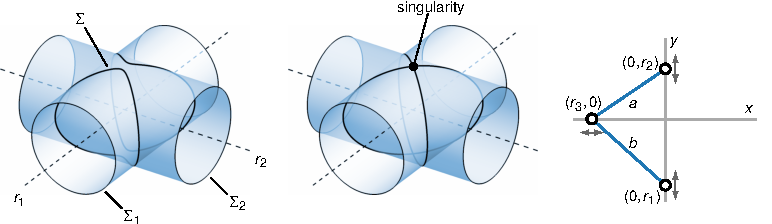
\includegraphics{frameworks/crank-slider.pdf}
  \end{center}
    \caption{Crank slider}
  \label{fig:crankslider}
\end{figure}

As $\Omega$ is an $(n-m)$-dimensional submanifold of $\mathbb{R}^n$, it is theoretically possible to find a smooth parameterization $\psi$ such that all points $\bar{\bm{r}} \in \Omega$ can be written as $\bar{\bm{r}} = \psi(\xi)$, where $\xi = (\xi_1, \xi_2, \ldots, \xi_{n-m}) \in \mathbb{R}^{n-m}$.
We also remark that one generally needs multiple such parameterizations to cover all points in $\Omega$.
The collective coordinates $\xi_i$ used to parameterize $\Omega$ could be any set of coordinates, although it is more convenient to choose coordinates physically relevant to the system.

It is also useful to analyze the intersection of level sets, say $\Omega_i$ and $\Omega_j$, locally at a point $\bar{\bm{r}} \in \Omega$.
If the Jacobian $\mathsf{J}$ is full rank, then its rows, i.e., the gradients $\nabla f_i$ of the constraint functions $f_i$, are independent.
Consequently, the tangent spaces $T_{\bar{\bm{r}}}{\Omega_i}$ and $T_{\bar{\bm{r}}}{\Omega_j}$---defined as sets of vectors perpendicular to $\nabla f_i$ and $\nabla f_j$---are different subspaces.
Since both tangent spaces are $(n-1)$-dimensional subspaces of $\mathbb{R}^n$, the fact they are different implies that (by dimension counting) $T_{\bar{\bm{r}}}{\Omega_i} + T_{\bar{\bm{r}}}{\Omega_j} = \mathbb{R}^n$.
In other words, $T_{\bar{\bm{r}}}{\Omega_i}$ and $T_{\bar{\bm{r}}}{\Omega_j}$ together generate (span) $\mathbb{R}^n$, and we say that the manifolds $\Omega_i$ and $\Omega_j$ are transverse to each other~\cite{guillemin1974}.
Hence, the Jacobian being full rank ensures that the level sets $\Omega_i$ of \emph{all} constraints are pairwise transverse.

Going back to our example, the configuration space $\Omega$ is composed of the curves obtained by the intersection of the cylinders $\Omega_1$ and $\Omega_2$.
When the cylinder radii satisfy $a < b$, then $\Omega$ is made up of two disconnected closed curves as illustrated in Fig.~\ref{fig:crankslider}(a).
Since $n = 3$ and $m=2$, $\Omega$ has a dimension equal to $n-m=1$, consistent with the fact that the curves are one dimensional.
The tangent spaces $T_{\bar{\bm{r}}}\Omega_1$ and $T_{\bar{\bm{r}}}\Omega_2$ for a point $\bar{\bm{r}} \in \Omega$ can be identified with the tangent planes of the two cylinders at that point.
It is clear that there is no point in $\Omega$ where the two cylinders share a common tangent plane and it can be shown (by direct computation) that Jacobian of the constraint map never drops rank.
Hence, the intersection shown in Fig.~\ref{fig:crankslider}(a) is indeed a transverse intersection.

More generally, there could be points $\bar{\bm{r}} \in \Omega$ where the Jacobian $\mathsf{J}(\bar{\bm{r}})$ is not full rank.
Such points are called \emph{singular points}.
If the Jacobian is rank deficient, at least two of its rows, say $\nabla f_i$ and $\nabla f_j$, are not independent and thus $T_{\bar{\bm{r}}}\Omega_i = T_{\bar{\bm{r}}}\Omega_j$.
By the arguments in the preceding paragraphs, this would also imply that the corresponding level sets $\Omega_i$ and $\Omega_j$ cannot be mutually transverse since $T_{\bar{\bm{r}}}\Omega_i + T_{\bar{\bm{r}}}\Omega_j \neq \mathbb{R}^n$.
Such a situation can be seen in our example when the two cylinders have the same radius, in which case $\Omega$ reduces to a self-intersecting curve.%
\footnote{An analogous situation arises while considering the intersection of a sphere and a cylinder.
If the sphere radius is equal to the cylinder diameter, the intersection curve $\Omega$ has a double point, and is called Viviani's curve~\cite{struik1988}.}
It is clear that the two cylinders share a common tangent plane at the point of self intersection.
Since the tangent spaces are not mutually independent at this point, they cannot possibly generate $\mathbb{R}^3$.

% TODO resolving branches are the singularity -- the tangent cone.

% TODO: talk about exceptions x^{3} - y^{3}, for instance.

To summarize, when a set of constraints are imposed on a mechanical system, its configuration space becomes nontrivial.
Singularities may occur in the configuration space at points where the Jacobian of the constraint map drops rank.
This means that, at these singular points, some of the constraints are equivalent to linear order.
Geometrically, this corresponds to nontransversal intersection of the zero level sets of the constraint functions at that point.

\section{Frameworks}

We consider bar-joint frameworks made of $N \geq 3$ point-like joints in $d$ dimensions connected by $m < Nd - \frac{1}{2}d(d+1)$ freely-rotating, massless bars.
If the joints have position vectors $\bm{r}_1, \bm{r}_2, \ldots, \bm{r}_{N} \in \mathbb{R}^d$ in the lab frame, the framework's configuration can be fully described at any given moment using a configuration vector $\bm{r}\in\mathbb{R}^{N d}$ defined by $\bm{r} = (\bm{r}_1, \bm{r}_2, \ldots, \bm{r}_{N})$.
Let the $i$th bar in the framework have a length $\ell_{i}$.
It is also clear that the length can always be considered as a function of the coordinate $\bm{r}$ describing the entire network, and we emphasize this by writing $\ell_i \equiv \ell_i(\bm{r})$.

As before, the configuration space of the framework is the set $\Omega$ such that the length of the $i$th bar $\ell_{i}$ is equal to its rest length $\bar{\ell}_{i}$.
Configurations in $\Omega$ are deformed states of the framework or the configurations obtained from such states after a rigid motion in $d$-dimensional space (i.e., after rotations, reflections, or translations).
To separate the actual deformations of the framework from trivial rigid motions, it is more useful to consider the shape space $\Sigma$, is the set of all configurations with distinct shapes, and
obtained after ``filtering out'' all the rigid motions from the configuration space.
More technically, the shape space is the quotient space $\Sigma = \Omega/SE(d)$, where $SE(d)$ is the special Euclidean group in $d$ dimensions~\cite{littlejohn1995}.

To practically identify $\Sigma$, we first switch to a Cartesian body frame attached to the framework so that all $\frac{1}{2}d(d+1)$ rigid motions are eliminated~\cite{herschbach1959,echenique2011}.
We require $n = Nd - \frac{1}{2}d(d+1)$ coordinates to specify the state of the framework in the body frame and let $\bm{q} \in \mathbb{R}^{n}$ be its configuration vector in this frame.
Now consider $m$ holonomic constraint functions $f_i: \mathbb{R}^{n} \to \mathbb{R},\,i=1,2,\ldots,m$, each associated with a single bar, and defined by
%
\begin{equation}
  f_i(\bm{q}) = \frac{\ell_i^2(\bm{q}) - \bar{\ell}_i^2}{2\bar{\ell}_i},
\end{equation}
%
where the factor of $1/(2\bar{\ell}_i)$ is for later convenience.
As before, the $m$ scalar constraint functions can also be considered together as a single constraint map $f: \mathbb{R}^{n} \to \mathbb{R}^m$ defined by $f(\bm{q}) = [f_1(\bm{q}), f_2(\bm{q}), \ldots, f_m(\bm{q})]$.
Then, the shape space is the zero level set $\Sigma = \left\{\bm{q} \in \mathbb{R}^{n}: f(\bm{q}) = \bm{0} \right\}$.
In the absence of external forces, each point in $\Sigma$ is a ground-state configuration of the framework with a distinct shape.

The compatibility matrix $\mathsf{C}(\bm{q})$~\cite{pellegrino1986,lubensky2015} at a configuration $\bm{q} \in \Sigma$ is the $m \times n$ Jacobian matrix $\nabla f$ of the constraint map $f$.
If $\mathsf{C}$ has full rank for all points in $\Sigma$, then $\Sigma$ is an $(n - m)$-dimensional submanifold of $\mathbb{R}^{n}$~\cite{leimkuhler2005,lee2013}.
When $\Sigma$ has a ``branched'' structure, e.g., like in Fig.~\ref{fig:4bar_cs}, $\mathsf{C}(\bm{q})$ drops rank at the singularity where the branches meet~\cite{lopez-custodio2020,muller2019}, and the constraints cease to be linearly independent.
Such singularities are the most common singularities~\cite{lopez-custodio2019,lopez-custodio2020} found in a framework and here we consider the situation where they occur only at isolated points of $\Sigma$.\footnote{For other, less common singularities that can occur in a framework, see Refs.~\cite{lopez-custodio2020,muller2019,muller2017}, and references therein.}
The branches of $\Sigma$, being $(n-m)$-dimensional submanifolds of $\mathbb{R}^{n}$, can be individually parameterized using a set of coordinates $\xi \in \mathbb{R}^{n-m}$, analogous to generalized coordinates, called shape coordinates~\cite{littlejohn1995} as they capture the shape changes of the framework as it moves on $\Sigma$.
We also assume that $n$ is small enough that such parameterizations can be found without much difficulty and that
the branches are linearly independent at the singularity~\cite{lopez-custodio2020}.

\subsection{Zero modes and self stresses}

Irrespective of whether or not $\mathsf{C}$ is full rank, we define a \emph{zero mode} to be a perturbation $\bm{v} \in \mathbb{R}^n$ that preserves the constraints to linear order, i.e., $\mathsf{C}\bm{v} = 0$ or $\bm{v} \in \ker \mathsf{C}$.
If $\mathsf{C}$ is full rank, then there is a well-defined tangent space $T_{\bar{\bm{q}}}\Sigma$ at $\bar{\bm{q}}$ and $\bm{v} \in T_{\bar{\bm{q}}} \Sigma$.
In such a situation, the number $z$ of zero modes is
%
\begin{equation}
  z = n - m\,,
\end{equation}
%
which is equal to the dimension of tangent space.
Zero modes include every infinitesimal perturbations of the framework that restricts $\bar{\bm{q}}$ to the shape space $\Sigma$.

However, like in the case of general constraints, the compatibility matrix $\mathsf{C}$ need not always be full rank.
If the compatibility matrix is not full rank, then this implies that its rows are not fully independent and there are $m$-dimensional nonzero vectors $\sigma \in \mathbb{R}^m$ such that
\begin{equation}
  \sigma\trans\mathsf{C}(\bar{\bm{q}}) = \bm{0}\,.\label{eq:selfstress}
\end{equation}
Any vector $\sigma$ that belongs to the left null space of the compatibility matrix has the physical interpretation of having components equal to  the signed magnitude of spring tensions that enforce static equilibrium of the framework.
For this reason, $\sigma$ is called a self stress.
Applying the rank-nullity theorem to the transpose of Eq.~\eqref{eq:selfstress} we find the number $s$ of self stresses to be
\begin{equation}
  s = m - \rank{\mathsf{C}\trans(\bar{\bm{q}})} = m - \rank{\mathsf{C}(\bar{\bm{q}})}\,.\label{eq:sscount}
\end{equation}
If the compatibility matrix $\mathsf{C}$ is not full rank at a point $\bar{\bm{q}}$, there is no well defined tangent space $T_{\bar{\bm{q}}}\Sigma$ at that point.
However, one can still count the number $z$ of zero modes by applying the rank-nullity theorem on $\mathsf{C}$, which gives
\begin{equation}
  z = n - \rank{\mathsf{C}(\bar{\bm{q}})}\label{eq:zmcount}\,.
\end{equation}
Eliminating $\rank{\mathsf{C}(\bar{\bm{q}})}$ from Eqs.~\eqref{eq:sscount} and \eqref{eq:zmcount} we arrive at the Maxwell--Calladine relation
%
\begin{equation}
  z - s = n - m\,,\label{eq:mcindex}
\end{equation}
%
which shows that the difference in the number of zero modes and the self stress at a point $\bar{\bm{q}} \in \Sigma$ depends only on the dimension $n$ of the configuration space and the number of constraints $m$.
Since we have assumed that $m \leq n$, we see that the presence of a self stress creates new zero modes.

% TODO: picture with constraint manifolds.
%
% \hl{TODO}
% \begin{figure}
%   \label{fig:tether}
%   \caption{A particle at the $\bar{\bm{q}} = (0,0)$ tethered to two parallel walls using two springs---a system that can support a state of self stress.  The shape spaces $\Sigma_1$ and $\Sigma_2$ of the two constraint functions share a common tangent space as illustrated.}
% \end{figure}

\section{Elastic energy of a framework}
\label{sec:energy}

The energy stored in the $i$th bar of the framework is a function $\phi_i(\ell_i)$ of its length $\ell_i$.
We additionally assume that this function has a minimum when $\ell_i = \bar{\ell_i}$, the natural length of the bar, for all bars.
The total energy of the framework is then
%
\begin{equation}
  U({\bm{q}}) = \sum_{i=1}^{m} \phi_i[\ell_i({\bm{q}})]\,.
\end{equation}
%
On the shape space $\Sigma$, the bars are at their natural lengths, i.e., for all points $\bar{\bm{q}} \in \Sigma$, $\ell_i(\bar{\bm{q}}) = \bar{\ell_i}$.
The bars are also at their minimum potential energies $\phi_i(\bar{\ell_i})$, which we assume to be zero for all bars without any loss of generality.
We first look at the lowest-order approximation to the energy, viz., the harmonic approximation.

\subsection{Harmonic approximation}

The $i$th bar in the framework has a potential energy $\phi_i[\ell_i(\bm{q})]$.
The constraint function associated with this bar is $f_i(\bm{q}) = [\ell_i^2(\bm{q}) - \bar{\ell}_i^2]/(2\bar{\ell}_i)$.
Consider a point $\bar{\bm{q}}$ on the shape space $\Sigma$ where the framework is in equilibrium.
Dropping the index $i$ for now and noting that $\ell(\bar{\bm{q}}) = \bar{\ell}$, we first express the gradient and the Hessian of the length $\ell(\bm{q})$ at $\bm{q} = \bar{\bm{q}}$ in terms of the gradient and the Hessian of $f(\bm{q})$ as
%
\begin{equation}
\begin{aligned}
  \partial_j \ell &= \partial_j f,\\
  \partial_j\partial_k \ell &= \partial_j\partial_k f - \bar{\ell}^{-2}\partial_j f\partial_k f,
  \label{sm:eq:lentomap}
\end{aligned}
\end{equation}
%
where all the partial derivatives are with respect to the components of $\bm{q}$ and evaluated at $\bm{q} = \bar{\bm{q}}$.

Since we have assumed the potential energy of all bars to have a minimum value (assumed to be zero) on the shape space, where $\ell = \bar{\ell}$, the derivative $\phi'(\bar{\ell})$ vanishes.
We wish to find the lowest-order expansion of the total potential energy $U(\bm{q})$ near a point $\bar{\bm{q}} \in \Sigma$.
First, let us consider the case where $\bar{\bm{q}}$ is not a point of self stress, in which case all zero modes are tangent to $\Sigma$ and can be extended to smooth deformations of the framework that do not cost energy to any order.
In such a situation, after setting $\bm{q} \to \bar{\bm{q}} + \bm{q}$, the potential energy of a single bar to $\mathscr{O}(\Abs{\bm{q}}^2)$ is the familiar Hookean potential
%
\begin{equation}
  \phi[\ell(\bar{\bm{q}} + \bm{q})] =  \frac{1}{2}\phi''(\bar{\ell})(\partial_j \ell\,q_j)^2 + \mathscr{O}(\Abs{\bm{q}}^3).
\end{equation}
%
Above, the partial derivatives of $\ell(\bm{q})$ and the derivatives of $\phi(\ell)$ have been evaluated at $\bar{\bm{q}} \in \Sigma$ and $\ell = \bar{\ell}$, respectively.
The repeated indices are summed over as usual.
Reintroducing the free index $i$, and noting that the stiffness $\kappa_{i} = \phi_{i}''(\ell_{i})$ and $\partial_{j}\ell_{i}\,q_{j} = \partial_{j}f_{i}\,q_{j} = \nabla f_{i}\cdot\bm{q}$, the total energy becomes
%
\begin{equation}
  U = \sum_{i=1}^m \phi_i[\ell_i(\bar{\bm{q}} + \bm{q})] \approx \frac{1}{2} \sum_{i=1}^m \kappa_i (\nabla f_i\cdot\bm{q})^2 = \frac{1}{2}\bm{q}\trans\mathsf{C}\trans\mathsf{K}\mathsf{C}\bm{q} = \frac{1}{2}\bm{q}\trans\mathsf{D}\bm{q}.
  \label{eq:regenergy}
\end{equation}
%
Here $\mathsf{D} = \mathsf{C}\trans\mathsf{K}\mathsf{C}$ is the dynamical matrix evaluated at $\bar{\bm{q}}$~\cite{lubensky2015} (assuming joints of unit mass) and $\mathsf{K}$ is the diagonal matrix of bar stiffnesses $\phi_{i}''(\bar{\ell}_{i})$, which we set equal to $\kappa$ for all bars for simplicity.

\subsection{Higher-order approximations}

Now let us analyze the case where there are additional zero modes due to the presence of a self stress.
Dropping the index $i$ again, we first expand the energy of a bar to $\mathscr{O}(\Abs{\bm{q}}^4)$ and find
%
\begin{equation}
  \begin{aligned}
    \phi[\ell(\bar{\bm{q}} + \bm{q})] &=
    \frac{1}{2}\phi''(\bar{\ell})(\partial_j \ell\,q_j)^2 +
    \frac{1}{6}\phi'''(\bar{\ell})(\partial_j \ell\,q_j)^3 +
    \frac{1}{2}\phi''(\bar{\ell})(\partial_j \ell\,q_j)\partial_k\partial_l \ell\, q_k q_l\\ &\qquad+
    \frac{1}{24}\phi''''(\bar{\ell})(\partial_j \ell\,q_j)^4 +
    \frac{1}{4}\phi'''(\bar{\ell})(\partial_j \ell\,q_j)^2 \partial_k \partial_l \ell\, q_k q_l\\ &\qquad+
    \frac{1}{8}\phi''(\bar{\ell})(\partial_j\partial_k \ell\, q_j q_k)^2 +
    \frac{1}{6}\phi''(\bar{\ell})(\partial_j \ell\, q_j)\partial_k\partial_l\partial_m \ell\, q_k q_l q_m + \mathscr{O}(\Abs{\bm{q}}^5).
  \end{aligned}
  \label{sm:eq:energyexp}
\end{equation}
%
The subspace of zero modes is $\ker\mathsf{C}$ and its orthogonal compliment in $\mathbb{R}^n$ is $(\ker\mathsf{C})^\perp$ and we write $\bm{q} = \bm{u} + \bm{v}$.
Here $\bm{u} \in \ker\mathsf{C}$ is a zero mode and $\bm{v} \in (\ker\mathsf{C})^{\perp}$ is a fast vibrational mode of the system.
First let us analyze the contribution of the zero mode $\bm{u}$ to the energy.
Since $\bm{u}$ is a zero mode, we have $\mathsf{C}\bm{u} = \bm{0}$.
Now, as $\partial_j f$ is a row of $\mathsf{C}$, this implies $\partial_j f u_j = 0$.
Using this in Eq.~\eqref{sm:eq:lentomap} we get
%
\begin{equation}
  \begin{aligned}
    \partial_j \ell\,u_j &= \partial_j f u_j=0,\\
    \partial_j \partial_k \ell\, u_j u_k
                        &= \partial_j\partial_k f u_j u_k - \bar{\ell}^{-2}(\partial_j f\, u_j) (\partial_k f\, u_k)\\
                        &= \partial_j\partial_k f\, u_j u_k.
  \end{aligned}
\end{equation}
%
Setting $\bm{v} = \bm{0}$ in the series expansion [Eq.~\eqref{sm:eq:energyexp}] and using the above simplifications, it is clear that the only nonvanishing contribution to the energy would come from the $\mathscr{O}(\Abs{\bm{u}}^4)$ term $\frac{1}{8}{\phi''(\bar{\ell})}(\partial_j \partial_k \ell\, u_j u_k)^2 = \frac{1}{8}{\phi''(\bar{\ell})}(\partial_j \partial_k f\, u_j u_k)^2$.

To understand how a fast mode $\bm{v}$ contributes to the energy, we similarly set $\bm{u} = \bm{0}$ in the energy expansion.
Since $\bm{v}$ belongs to the orthogonal compliment of the subspace of zero modes, by definition, $\partial_j \ell v_j = \partial_j f v_j \ne 0$.
Hence, we see that the first nonvanishing contribution comes from the $\mathscr{O}(\Abs{\bm{v}}^2)$ term $\frac{1}{2}\phi''(\bar{\ell})(\partial_j \ell\, v_j)^2 = \frac{1}{2}\phi''(\bar{\ell})(\partial_j f\, v_j)^2$.
This shows that the energy scales as $\mathscr{O}(\Abs{\bm{u}}^4) \sim \mathscr{O}(\Abs{\bm{v}}^2)$, i.e., zero and fast modes respectively make quartic- and harmonic-order contributions to the energy.
Finally, we set $\bm{q} = \bm{u} + \bm{v}$ in Eq.~\eqref{sm:eq:energyexp}, and find the energy of the $i$th bar to the lowest order in $\bm{u}$ and $\bm{v}$ as
%
\begin{equation}
  \begin{aligned}
    \phi_i &= \frac{1}{2}\phi_i''(\bar{\ell}_i)(\partial_j\, f_i\, v_j)^2 + \frac{1}{2}\phi''_i(\bar{\ell}_i)(\partial_j f_i\, v_j)(\partial_k \partial_l f_i\, u_k u_l) + \frac{1}{8}\phi''_i(\bar{\ell}_i)(\partial_k \partial_l f_i\, u_k u_l)^2\\
           &\qquad+ \mathscr{O}(\Abs{\bm{u}}^5) + \mathscr{O}(\Abs{\bm{u}}^{3}\Abs{\bm{v}}) +\mathscr{O}(\Abs{\bm{u}}\Abs{\bm{v}}^{2}),
  \end{aligned}
\end{equation}
%
where we have reintroduced the free index $i$.
In the above equation, $\phi_{i}''(\bar{\ell}_i) = \kappa_i$, the stiffness of the $i$th bar, $\partial_j f_i v_j = \nabla f_i\cdot\bm{v}$, and $\partial_k\partial_l f_i\, u_k u_l = \bm{u}\trans(\hess f_i)\bm{u}$, with $\hess f_i$ being the Hessian matrix of the $i$th constraint function $f_i$.
Then, the energy of the $i$th bar to the lowest order is
%
\begin{equation}
  \phi_i \approx \frac{1}{2}\kappa_i \left[\nabla f_i\cdot\bm{v} + \frac{1}{2}\bm{u}\trans(\hess f_i)\bm{u}\right]^2.
\end{equation}
%
Recognizing that $\frac{1}{2}\bm{u}\trans(\hess f_{i})\bm{u}$ is the $i$th component of the column vector $\bm{w}(\bm{u}) \in \mathbb{R}^{m}$ defined in the main text, the total energy to the lowest order in $\bm{u}$ and $\bm{v}$ takes the form
%
\begin{equation}
  U = \sum_{i=1}^m \phi_i \approx \frac{1}{2} [\mathsf{C}\bm{v} + \bm{w}(\bm{u})]\trans\,\mathsf{K}\,[\mathsf{C}\bm{v} + \bm{w}(\bm{u})].
  \label{eq:energy_singular}
\end{equation}
%
This equation is a generalization of the energy of harmonic spring networks~\cite{zhang2016,woodhouse2018} and colloidal clusters~\cite{kallus2017} that have zero modes, for an arbitrary number of zero modes and degrees of freedom, as well as a general interaction energy $\phi_{i}$ between the particles (i.e., the joints).
